\begin{appendices}
\addcontentsline{toc}{section}{Appendices}


%\section{The Flux Sketch}
%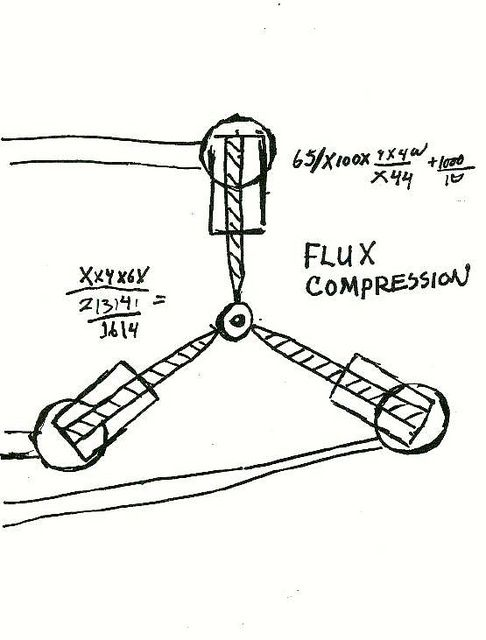
\includegraphics[width=\textwidth]{Report/Appendices/flux_sketch.jpg}
%\label{appx: Flux Sketch}


\section{Data-set Manipulation}

\subsection{CSV Combiner Script}
\label{appx: CSV Combiner Script}
\begin{lstlisting}
#!/bin/bash

# Input Directory
input_dir="../Malware"

cd "$input_dir"

# Set the output file name
output_file="combined.csv"

# Check if the output file already exists and delete it
if [ -f "$output_file" ]; then
  rm "$output_file"
fi

# Print a status message
echo "Combining files..."

# Loop through all the files that match the pattern reduced_*.csv
for file in $(ls *.csv | sort -V)
do
  # Check if the file exists
  if [ -f "$file" ]; then
    # Print a status message
    echo "Combining $file..."

    # If this is the first file, copy the header to the output file
    if [ ! -f "$output_file" ]; then
      head -n 1 "$file" > "$output_file"
    fi

    # Append all the rows except the header to the output file
    tail -n +2 "$file" >> "$output_file"
  fi
done

# Print a status message
echo "Done."
\end{lstlisting}

\newpage
\subsection{Feature Extraction \& Reduction}
\label{appx: Feature Extraction}

\begin{lstlisting}
# Define the columns you want to keep
cols_to_use = ['frame.len', 'radiotap.dbm_antsignal', 'radiotap.length', 'wlan.duration',
                   'wlan_radio.duration', 'wlan_radio.signal_dbm', 'radiotap.present.tsft',
                   'wlan.fc.type', 'wlan.fc.subtype', 'wlan.fc.ds', 'wlan.fc.frag',
                   'wlan.fc.moredata', 'wlan.fc.protected', 'wlan.fc.pwrmgt', 'wlan.fc.retry',
                   'wlan_radio.phy', 'udp.length', 'ip.ttl', 'arp', 'arp.proto.type',
                   'arp.hw.size', 'arp.proto.size', 'arp.hw.type', 'arp.opcode',
                   'tcp.analysis', 'tcp.analysis.retransmission', 'tcp.option_len',
                   'tcp.checksum.status', 'tcp.flags.ack', 'tcp.flags.fin', 'tcp.flags.push',
                   'tcp.flags.reset', 'tcp.flags.syn', 'dns', 'dns.count.queries', 'dns.count.answers',
                   'dns.resp.len', 'dns.resp.ttl', 'http.request.method', 'http.response.code',
                   'http.content_type', 'ssh.message_code', 'ssh.packet_length', 'nbns',
                   'nbss.length', 'nbss.type', 'ldap', 'smb2.cmd', 'smb.flags.response',
                   'smb.access.generic_read', 'smb.access.generic_write', 'smb.access.generic_execute','Label']

# Define the chunk size you want to read in each iteration
batch_size = 1000000

# Initialize an empty dataframe to hold the combined results
combined_df = pd.DataFrame()

# Iterate through the file in batches
for chunk in pd.read_csv('botnet_combined.csv', chunksize=batch_size, usecols=cols_to_use, low_memory=False):
    
    # Combine the processed chunk with previous chunks
    combined_df = pd.concat([combined_df, chunk])
\end{lstlisting}

\newpage
\begin{lstlisting}
# Drop all missing rows that contain only nan values
combined_df = combined_df.dropna(how='all')

# Drop all rows with missing values in Label Column
combined_df = combined_df.dropna(subset=['Label'])

# Fill NAs with zeros
# Change nan values to 0
combined_df = combined_df.fillna(0)
\end{lstlisting}

\begin{lstlisting}
# Duplicate the dataframe
df = combined_df.copy()

# Regex to keep only the first value e.g 
# -100-100-10 becomes -100,   123-456-1 becomes 123, -10-2 becomes-10, 81-63-63 becomes 81
def seperated_values(x):
    x = str(x)
    match = re.match(r'^(-?\d+).*$', x)
    if match:
        return match.group(1)
    else:
        return x

# Go through all columns and change seperate values into just one value
for column in df.columns:
    df[column] = df[column].apply(seperated_values)
    print('Processing', column)
print('Done')

# Find Rows that contain values such as Oct-26, Oct-18, Feb-10 etc.. as these appear to be invalid and we will drop these rows.
regex = r"\b(?:\d{2}|(?:Jan|Feb|Mar|Apr|May|Jun|Jul|Aug|Sep|Oct|Nov|Dec))-(?:\d{2}|(?:Jan|Feb|Mar|Apr|May|Jun|Jul|Aug|Sep|Oct|Nov|Dec))\b"

# Use str.match method to apply the regex pattern to the column
mask = df['tcp.option_len'].astype(str).str.match(regex).fillna(False)
df = df[~mask]

mask = df['dns.resp.ttl'].astype(str).str.match(regex).fillna(False)
df = df[~mask]

mask = df['ip.ttl'].astype(str).str.match(regex).fillna(False)
df = df[~mask]

mask = df['smb2.cmd'].astype(str).str.match(regex).fillna(False)
df = df[~mask]

df.to_csv('Botnet_Reduced.csv', index=False)    

\end{lstlisting}

\newpage

\section{Conda Environments}
\label{appx: Conda_Env}

\subsection{Neural Networks - Apple Silicon}

\begin{lstlisting}
conda create -n nn-env python=3.9
conda activate nn-env
conda install -c apple tensorflow-deps
conda install -c conda-forge -y pandas jupyter
pip install tensorflow-macos==2.10
pip install numpy, matplotlib, scikit-learn, scipy, seaborn
\end{lstlisting}

\subsection{Classifiers}

\begin{lstlisting}
# Conda environment used for Random Forest, XGBoost and K-NN.

conda create -n ml-env python=3.9
conda activate ml-env
conda install -c conda-forge -y pandas jupyter
pip install numpy, matplotlib, scikit-learn, scipy, seaborn, xgboost
\end{lstlisting}

\newpage

\section{Data Preprocessing}
\label{appx:Data Processing}

\subsection{MinMax Scaling}
\label{appx:Scaling}

\begin{lstlisting}
# Define the scaler
scaler = MinMaxScaler()

# Fit the scaler to the following columns we define
scale_cols = [
        'frame.len',
        'radiotap.dbm_antsignal', 
        'radiotap.length', 
        'wlan.duration', 
        'wlan_radio.duration', 
        'wlan_radio.signal_dbm',
        'ip.ttl', 
        'udp.length', 
        'nbss.length',
        'dns.count.answers', 
        'dns.count.queries',
        'dns.resp.ttl',
        'ssh.packet_length']
        
# Fit the X_train and X_test
X_train[scale_cols] = scaler.fit_transform(X_train[scale_cols])
X_test[scale_cols] = scaler.transform(X_test[scale_cols])
\end{lstlisting}

\subsection{OHE Encoding}
\label{appx:OHE Encoding}
\begin{lstlisting}
cols_to_encode = [col for col in X_train.columns if col not in scale_cols]
X_all = pd.concat([X_train, X_test], axis=0)

X_all_ohe = pd.get_dummies(X_all, columns=cols_to_encode, drop_first=True, dtype=np.uint8)

# split back into train and test sets
X_train_ohe = X_all_ohe[:len(X_train)]
X_test_ohe = X_all_ohe[len(X_train):]
\end{lstlisting}

\newpage
\subsection{Label Encoding}
\label{appx:Label Encoding}
\begin{lstlisting}
    # Use Label Encoder to encode the target variable
le = LabelEncoder()

label_encoder = le.fit(y_train)
y_train_encoded = label_encoder.transform(y_train)
\end{lstlisting}

\subsection{Loading Dataset}
\label{appx:Loading Dataset}
\begin{lstlisting}
chunk_size = 1000000
dtype_opt = {
    'frame.len': 'int64',
    'radiotap.dbm_antsignal': 'int64',
    'radiotap.length': 'int64',
    'radiotap.present.tsft': 'int64',
    'wlan.duration': 'int64',
    'wlan.fc.ds': 'int64',
    'wlan.fc.frag': 'int64',
    'wlan.fc.moredata': 'int64',
    'wlan.fc.protected': 'int64',
    'wlan.fc.pwrmgt': 'int64',
    'wlan.fc.type': 'int64',
    'wlan.fc.retry': 'int64',
    'wlan.fc.subtype': 'int64',
    'wlan_radio.duration': 'int64',
    'wlan_radio.signal_dbm': 'int64',
    'wlan_radio.phy': 'int64',
    'arp': 'object',
    'arp.hw.type': 'object',
    'arp.proto.type': 'int64',
    'arp.hw.size': 'int64',
    'arp.proto.size': 'int64',
    'arp.opcode': 'int64',
    'ip.ttl': 'int64',
    'tcp.analysis': 'int64',
    'tcp.analysis.retransmission': 'int64',
    'tcp.checksum.status': 'int64',
    'tcp.flags.syn': 'int64',
    'tcp.flags.ack': 'int64',
    'tcp.flags.fin': 'int64',
    'tcp.flags.push': 'int64',
    'tcp.flags.reset': 'int64',
    'tcp.option_len': 'int64',
    'udp.length': 'int64',
    'nbns': 'object',
    'nbss.length': 'int64',
    'ldap': 'object',
    'smb2.cmd': 'int64',
    'dns': 'object',
    'dns.count.answers': 'int64',
    'dns.count.queries': 'int64',
    'dns.resp.ttl': 'int64',
    'http.content_type': 'object',
    'http.request.method': 'object',
    'http.response.code': 'int64',
    'ssh.message_code': 'int64',
    'ssh.packet_length': 'int64'
}

# Read the data
print('Reading X...')
X = pd.DataFrame()
for chunk in pd.read_csv('X.csv', chunksize=chunk_size, usecols=dtype_opt.keys(), dtype=dtype_opt, low_memory=False):
    X = pd.concat([X, chunk])

print('Reading y...')
y = pd.DataFrame()
for chunk in pd.read_csv('y.csv', chunksize=chunk_size, usecols=['Label'], dtype='object', low_memory=False):
   y = pd.concat([y, chunk])

# Split the data into training and testing sets
print('Splitting the data...')
X_train, X_test, y_train, y_test = train_test_split(X, y, test_size=0.30, random_state=1234, stratify=y)
\end{lstlisting}

\newpage
\section{Classifiers}
\label{appx: Classifiers}

\subsection{Base K-Nearest Neighbor (KNN)}
\begin{lstlisting}
# Use KNN
from sklearn.neighbors import KNeighborsClassifier

k=5

# Create KNN classifier
knn = KNeighborsClassifier(n_neighbors=k, n_jobs=-1)

# Fit the model
knn.fit(X_train_ohe, y_train_encoded)

# predict the test set
y_knn_pred = knn.predict(X_test_ohe)

from sklearn.metrics import classification_report, roc_auc_score

# Get the classification report
report = classification_report(y_test_encoded, y_knn_pred)

print('Classification Report:\n', report)

# Get the all the metrics for the multi class classification

print('Accuracy: ', accuracy_score(y_test_encoded, y_knn_pred))
print('Precision: ', precision_score(y_test_encoded, y_knn_pred, average='macro'))
print('Recall: ', recall_score(y_test_encoded, y_knn_pred, average='macro'))
print('F1 Score: ', f1_score(y_test_encoded, y_knn_pred, average='macro'))

# Get the confusion matrix for multi-class and plot it
confusion = confusion_matrix(y_test, y_rf_pred)
print('Confusion Matrix\n')
print(confusion)

# Plot the confusion matrix for multi-class classification using seaborn
labels = ['Normal', 'SSDP', 'Website Spoofing', 'Malware', 'Botnet', 'SSH', 'SQL Injection']

plt.figure(figsize=(8, 8))
sns.heatmap(confusion, annot=True, fmt='d', cmap='Blues', xticklabels=labels, yticklabels=labels)
plt.title('Confusion Matrix')
plt.xlabel('Predicted')
plt.ylabel('Actual')
plt.show()

plt.figure(figsize=(10, 10))
feat_importances = pd.Series(rf.feature_importances_, index=X_train_ohe.columns)
feat_importances.nlargest(20).plot(kind='barh')
plt.show()
\end{lstlisting}

\subsection{XGBoost}

\subsubsection{Base XGBoost CF}
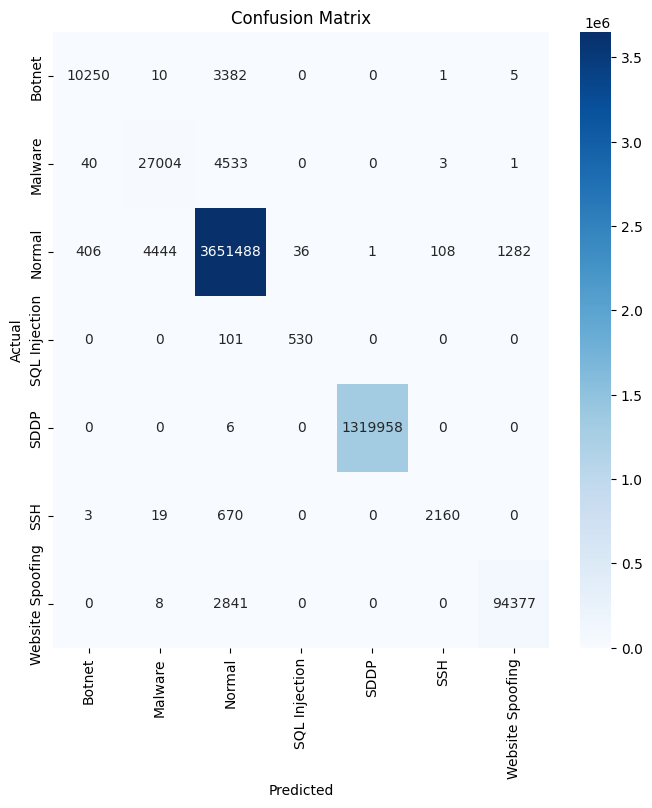
\includegraphics[width=\textwidth]{Appendices/Base_XGB_CF.png}
\newpage

\subsubsection{Base XGBoost Classification Report}
\begin{lstlisting}
                  precision    recall  f1-score   support

           0       0.96      0.75      0.84     13648
           1       0.86      0.86      0.86     31581
           2       1.00      1.00      1.00   3657765
           3       0.94      0.84      0.89       631
           4       1.00      1.00      1.00   1319964
           5       0.95      0.76      0.84      2852
           6       0.99      0.97      0.98     97226

    accuracy                           1.00   5123667
   macro avg       0.96      0.88      0.91   5123667
weighted avg       1.00      1.00      1.00   5123667
\end{lstlisting}

\newpage


\newpage



\section{Neural Networks}
\label{appx: Neural Networks}

\subsection{MLP NN v1}
\label{appx: MLP NN v1}

\begin{lstlisting}
# Create a sequential model
model = Sequential()
input_shape = (X_train_ohe.shape[1],)

# Add layers to the model
model.add(Dense(128, activation='relu', input_shape=input_shape))
model.add(Dense(64, activation='relu'))
model.add(Dense(7, activation='softmax'))

# Compile the model
model.compile(loss='categorical_crossentropy', optimizer='adam', metrics=['accuracy'])

# Train the model
model.fit(X_train_ohe, y_train_ohe, epochs=10, batch_size=32, validation_data=(X_test_ohe, y_test_ohe))

# Evaluate the model using test data
test_loss, test_acc = model.evaluate(X_test_ohe, y_test_ohe)

print('Test accuracy:', test_acc)
\end{lstlisting}

\subsubsection{MLP Neural Network}
\label{appx: MLP NN}

\begin{lstlisting}
from keras.models import Sequential
from keras.layers import Dense, Dropout, BatchNormalization
from keras.optimizers import SGD
from keras.initializers import he_uniform
from keras.metrics import AUC

# Define the number of classes
num_classes = 7

# Define the model architecture
model = Sequential()

# Add the input layer
model.add(Dense(100, input_shape=(X_train_ohe.shape[1],), activation='relu', kernel_initializer=he_uniform()))

# Add batch normalization
model.add(BatchNormalization())

# Add the first hidden layer
model.add(Dense(80, activation='relu', kernel_initializer=he_uniform()))
model.add(Dropout(0.25))
model.add(BatchNormalization())

# Add the second hidden layer
model.add(Dense(60, activation='relu', kernel_initializer=he_uniform()))
model.add(Dropout(0.2))
model.add(BatchNormalization())

# Add the third hidden layer
model.add(Dense(40, activation='relu', kernel_initializer=he_uniform()))
model.add(BatchNormalization())

# Add the fourth hidden layer
model.add(Dense(20, activation='relu', kernel_initializer=he_uniform()))
model.add(BatchNormalization())

# Add the output layer
model.add(Dense(num_classes, activation='softmax'))

# Define the optimizer
sgd = SGD(lr=0.01, momentum=0.9)

# Compile the model
model.compile(loss='categorical_crossentropy', optimizer=sgd, metrics=[AUC()])

# Train the model
batch_size = 170
epochs = 10
history = model.fit(X_train_ohe, y_train_ohe, batch_size=batch_size, epochs=epochs, validation_data=(X_test_ohe, y_test_ohe))

# Evaluate the model on your test data
test_loss, test_auc = model.evaluate(X_test_ohe, y_test_ohe)
\end{lstlisting}



\end{appendices}


